\documentclass[oneside]{VUMIFPSkursinis}
\usepackage{algorithmicx}
\usepackage{algorithm}
\usepackage{algpseudocode}
\usepackage{amsfonts}
\usepackage{float}
\usepackage{amsmath}
\usepackage{bm}
\usepackage{caption}
\usepackage{color}
\usepackage{float}
\usepackage{graphicx}
\usepackage{listings}
\usepackage{subfig}
\usepackage{tabularx}
\usepackage{wrapfig}
\newcolumntype{P}[1]{>{\centering\arraybackslash}p{#1}}
\usepackage[%  
    colorlinks=true,
    linkcolor=black
]{hyperref}
\university{Vilniaus universitetas}
\faculty{Matematikos ir informatikos fakultetas}
\department{Programų sistemų katedra}
\papertype{}
\title{Virtualios ir realios mašinos modelis}
\titleineng{Virtual and real machine model}
\status{2 kurso 3 grupės studentai}
\author{Matas Savickis}
\secondauthor{Justas Tvarijonas}  
\thirdauthor{Greta Pyrantaitė}   
\supervisor{Mantas Grubliauskas Lekt.}
\date{Vilnius – \the\year}


\bibliography{bibliografija}

\begin{document}
\maketitle
\tableofcontents

\section{Reali mašina}
\begin{figure}[H]
		\centering	
	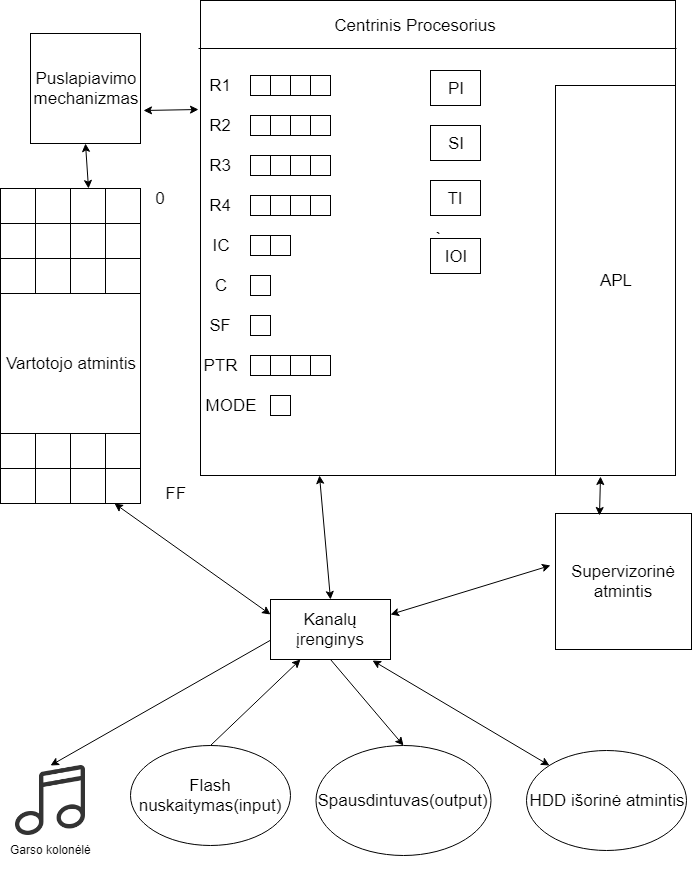
\includegraphics[width=18cm,height=20cm,keepaspectratio]{RealiMasina.png}
	\caption{Reali mašina}
	\label{fig:Reali mašina}
\end{figure}

\pagebreak

\subsection{Techninės įrangos elementai sudarantys realią mašiną}
\begin{itemize}
	\item{Centrinis procesorius}
	\item{Vartotojo atmintis}
	\item{Supervizorinė atmintis}
	\item{Išorinė atmintis}
	\item{Duomenų perdavimo kanalai}
	\item{Įvedimo įrenginys - flash atmintinis}
	\item{Išvedimo įrenginys - spausdintuvas}
	\item{Puslapiavimo mechanizmas}
\end{itemize}

\subsection{Centrinis procesorius}
	Centrinio procesoriaus paskirtis yra skaityti komandas iš atminties ir jas interpretuoti. Procesorius gali dirbti dviem rėžimais - supervizoriaus ir vartotojo. Supervizoriaus rėžime komandos yra apdorojamos aukšto lygio procesoriaus. Komandos vykdomos supervizoriaus režime yra skirtos operacinės sistemos funkcionavimui palaikyti. Procesorius persijungia į šį rėžimą pertaukimais arba sisteminiais kreipiniais.
\subsection{Procesoriaus registrai}
\begin{itemize}
	\item{R1, R2, R3, R4 - 4 baitų bendros paskirties registrai}
	\item{DS - registras rodantis duomenų segmento adresą}
	\item{CS - registras rodantis kodo segmento adresą}
	\item{IC - 2 baitų komandų skaitiklis}
	\item{C - 1 baito loginis registras (TRUE arba FALSE)}
	\item{SF - 1 baito požymių registras CF OF XX XXXZF - carry flag, overflow flag, zero flag}
	\item{PTR - 4 baitų puslapių lentelės registras(naudojamo puslapių lentelės numeris)}
	\item{MODE - registras, kurio reikšmė nusako procesoriaus darbo režimą(supervizorinis, vartotojo)}
	\item{PI - programinių pertraukimų registras}
	\item{SI - supervizorinių pertraukimų registras}
	\item{TI - taimerio registras}
	\item{CHST[1]...CHST[3] - kanalų būsenos registrai }
	\item{IOI - 2 baitų įvedimo ir išvedimo pertraukimų registras}
\end{itemize}

\subsection{Atmintys}
Pagrindinę realios mašinos atmintį dalinasi vartotojo ir supervizorinė atmintis. Kaskart sukuriant naują virtualią mašiną panaudojama dalis realios mašinos atminties. Atminties dydis 16 blokų po 16 žodžių. Žodžio ilgis 4 baitai. Supervizorinę atmintį naudoja aukšto lygio procesorius, tačiau šios atminties savo rašomoje programoje nenaudosim. Taip pat yra išorinė atmintis kietojo disko pavidalu.

\subsection{I/O}
Komandų įvedimui naudojamas ,,flash atmintinių" nuskaitymo įrenginys. Išvedimui naudojamas spausdintuvas.

\subsection{Puslapiavimo mechanizmas}
Puslapiavimo mechanizmas yra metodas skirtas virtualios atminties adreso parodymui į realios atminties adresą. Kiekvienai virtualiai mašinai skiriama 4 atminties blokai. Paskutinis lentelės blokas yra užpildomas realiais adresais. Naudojamas PTR(4 baitų a0,a1,a2,a3) registras kuriame laikomas puslapių lentelės bloko realūs adresai. Pagal a2 ir a3 baitus surandame bloką. Pagal virtualaus adreso x1 ir x2 yra nustatomas puslapis. Bloko adresas kur x1 randamas [4*(4*a2 a3)+x1], o prie bloko adreso pridėjus x2 gauname virtualų adresą: 4*[4*(4*a2 a3)+x1]x2.

\subsection{Duomenų perdavimo kanalai}
Skirti I/O ir atminties valdymui. Modelyje egzistuoja trys kanalai iš kurie kiekvienas atsakingas už skirtingus dalykus. Kanale vyksta arba rašymas arba skaitymas ir pabaigęs darbąą jis informuoja centrinį procesorių ir sukelia pertraukimą padidindamas IOI registro reikšmę. Kanalų būsenos yra saugomos CHST[1]...CHST[3] registruose.





\section{Virtuali mašina}

\subsection{Funkcija}
Virtuali mašina yra skirta paslepti realios mašinos sudėtingumą ir suteikti vartotojui instrukcijų sąrašą su kuriuo jis galėtų dirbti. Todėl operacinės sistemos paskirtis ir yra paslėpti realią mašiną ir duoti mums virtualią. Virtuali mašina taip pat suteikia darbų pasidalijimą kurio dėk galima paleisti kelias virtualias mašinas ir tokiu būdu ant kiekvienos iš jų atlikti skirtingas užduotis.

 \subsection{Modeliuojamos virtualios mašinos loginių komponentų aprašymas}
	\subsubsection{Atmintis}
	\begin{figure}[H]
		\centering	
	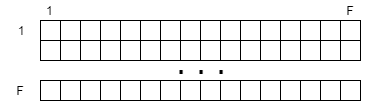
\includegraphics[width=18cm,height=20cm,keepaspectratio]{VMAtmintis.png}
	\caption{Virtualios mašinos atmintis}
	\label{fig:Virtualios mašinos atmintis}
\end{figure}

	Virtualios mašinos atmintis susideda iš 4 blokų po 16 žodžių iš viso 64 žodžiai po 4 baitus arba 32 bitus. Pirmi du atminties blokai bus paskirti duomenų segmentui(DS), o paskutiniai du blokai kodo segmentui(CS). Norint pasinaudoti puslapiavimo mechanizmu pirmas blokas bus išskiriamas surašyti realiems adresams. Naudosime registrą PTR(4 baitai a0 a1 a2 a3) kuriame laikomas puslapių lentelės bloko realūs adresai. Per a2 ir a3 surandame bloką. Pagal x1 ir x2 nustatomas puslapis. Bloko adresas, kur yra x1 randamas pagal formulę [4*(4*a2 a3)+x1]x2, o prie bloko adreso pridėjus x2 gauname vistualų adresą 4*[4*(4*a2 a3)+x1]x2 .Efektyviai naudotis Virtualia atmintimi įvesime du papildomus registus DS ir CS. DS registro reikšmė bus rodyklė į duomenų segmento atmintį, o CS reišmė rodyklė į kodo segmento atmintė.

	\subsubsection{Procesorius}
\begin{figure}[H]
		\centering	
	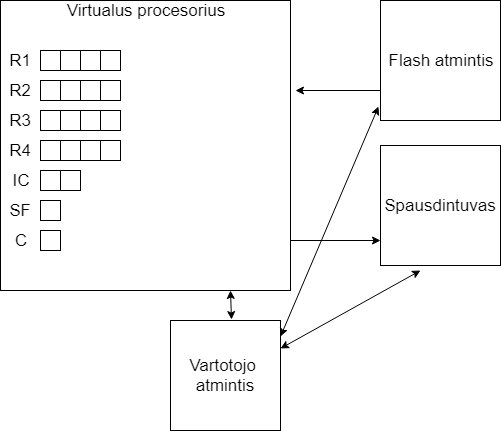
\includegraphics[width=18cm,height=20cm,keepaspectratio]{VMProcesorius.png}
	\caption{Virtualios mašinos procesorius}
	\label{fig:Virtualios mašinos procesorius}
\end{figure}
Registrai:
\begin{itemize}
	\item{R1...R4 - Bendros paskirties registrai}
	\item{IC - komandos skaitliukas, rodo sekančios komandos adresą }
	\item{SF - status flagas rodantis programos būseną}
	\item{C - loginis registras(TRUE arba FALSE)}
	\item{DS - rodo į duomenų segmentą atmintyje}
	\item{CS - rodo į kodo segmentą atmintyje}
\end{itemize}

	
	





\end{document}